\begin{pastexam}[label={px:df3-113-ds-02}]{地方三等資訊處理 113 年 第二題}
（申論；25 分）

請回答下列關於二元樹（Binary Tree）的問題：
\begin{enumerate}[leftmargin=2.6em, labelsep=0.4em]
\item[㈠] 一個算術運算式（Arithmetic Expression）可以用一個二元樹表示，稱為算術運算樹（Expression Tree），
請將下列算術運算式以算術運算樹表示。（5 分）

$(\,(\,(\,5 + 1\,) \times 3 \;-\; (7 + 2\,)\,)\,/\,(\,(\,(\,2 \times 8\,) + 5\,)\,/\,7\,)\,)$
\item[㈡] 請判斷下列敘述是否正確：（5 分）

“一個算術運算樹是一個滿二元樹（Full Binary Tree, or Proper Binary Tree）”
\item[㈢] 子題㈠中的算術運算式是何種順序的運算表示式？請利用其算術運算樹將此運算式表示為一前序表示式
（Preorder Expression），並說明其過程。（5 分）
\item[㈣] 請敘述如何以子題㈠的算術運算樹計算出算術運算式的值，並逐步表示其過程。（10 分）
\end{enumerate}
\end{pastexam}

\begin{pastsoln}
\textbf{㈠} 運算式樹（資結書第~7.7~節）：內部節點是運算子，兩個子樹是它的左、右運算元；葉節點是數字。
由最外層的括號往內拆：最外層是「$\ldots / \ldots$」，左邊 $(5 + 1) \times 3 - (7 + 2)$，右邊
$((2 \times 8) + 5) / 7$；兩邊再各自拆下去。
\begin{center}
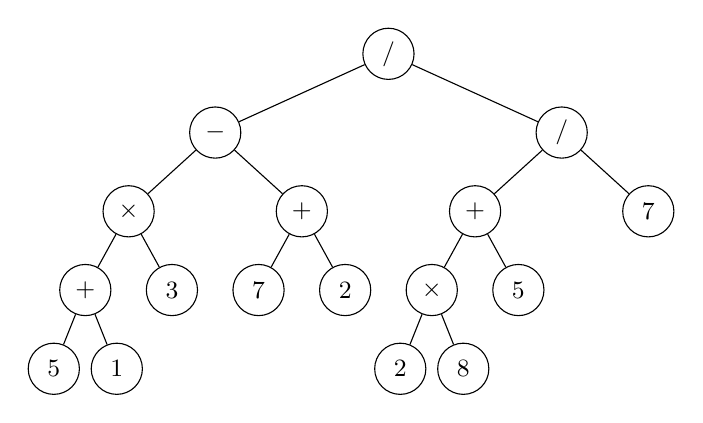
\begin{tikzpicture}[n/.style={circle,draw,inner sep=0pt,minimum size=6.5mm,font=\small},
  level distance=10mm, level 1/.style={sibling distance=44mm}, level 2/.style={sibling distance=22mm},
  level 3/.style={sibling distance=11mm}, level 4/.style={sibling distance=8mm}]
\node[n] {$/$}
  child {node[n] {$-$}
    child {node[n] {$\times$} child {node[n] {$+$} child {node[n] {5}} child {node[n] {1}}} child {node[n] {3}}}
    child {node[n] {$+$} child {node[n] {7}} child {node[n] {2}}}}
  child {node[n] {$/$}
    child {node[n] {$+$} child {node[n] {$\times$} child {node[n] {2}} child {node[n] {8}}} child {node[n] {5}}}
    child {node[n] {7}}};
\end{tikzpicture}
\end{center}
樹的中序走訪（每個子樹外面加括號）就還原出原來的運算式。

\textbf{㈡} 正確（就這題的四則運算而言）。 滿二元樹在這裡指 full／proper binary tree：每個節點的子節點數
是 $0$ 或 $2$。 算術運算式裡的 $+$、$-$、$\times$、$/$ 都是\textbf{二元運算子}，每個運算子恰有左、右兩個
運算元，所以每個內部節點恰有兩個子節點；數字（運算元）沒有子節點，是葉節點。 因此運算式樹是滿二元樹，
而且葉節點數比內部節點數多 $1$（資結書定理~7.2：$n_0 = n_2 + 1$）；上圖有 $8$ 個運算子、$9$ 個數字。
要注意的例外：運算式裡若有\textbf{一元}運算子（例如負號 $-x$），那個節點只有一個子節點，樹就不是
滿二元樹。 題目的運算式沒有一元運算子。

\textbf{㈢} 原運算式是\textbf{中序}（infix）表示式：運算子寫在兩個運算元中間，所以需要括號來指定順序。
前序表示式用前序走訪（資結書第~7.3~節）：先輸出根，再走左子樹，再走右子樹，遞迴進行。
\begin{itemize}
\item 根 $/$，接著走左子樹（根 $-$）：輸出 $-$；再走它的左子樹（根 $\times$）：輸出 $\times$，再走 $+$：輸出
$+\; 5\; 1$，回到 $\times$ 的右子 $3$；回到 $-$ 的右子樹：輸出 $+\; 7\; 2$。 左半部得到
$-\;\times\;+\;5\;1\;3\;+\;7\;2$。
\item 走右子樹（根 $/$）：輸出 $/$，左子樹 $+$：輸出 $+\;\times\;2\;8\;5$；右子 $7$。 右半部得到
$/\;+\;\times\;2\;8\;5\;7$。
\end{itemize}
合起來，前序表示式是
\[
/ \;\; - \;\; \times \;\; + \;\; 5 \;\; 1 \;\; 3 \;\; + \;\; 7 \;\; 2 \;\; / \;\; + \;\; \times \;\; 2 \;\; 8 \;\; 5 \;\; 7
\]
前序（和後序）表示式不需要括號，順序由運算子的位置唯一決定。

\textbf{㈣} 用\textbf{後序走訪}計算：一個運算子節點要等兩個子樹的值都算出來，才能計算自己。 遞迴寫法：
\begin{pseudo}{運算式樹求值}
\Function{Eval}{$x$}
    \If{$x$ 是葉節點}
        \State \Return $x$ 的數值
    \EndIf
    \State $a \gets$ \Call{Eval}{$x.\mathit{left}$}
    \State $b \gets$ \Call{Eval}{$x.\mathit{right}$}
    \State \Return $a \mathbin{\mathit{op}} b$ \Comment{$\mathit{op}$ 是 $x$ 存的運算子}
\EndFunction
\end{pseudo}
後序走訪的順序是 $5\;1\;+\;3\;\times\;7\;2\;+\;-\;2\;8\;\times\;5\;+\;7\;/\;/$，每遇到一個運算子就用
它的兩個子樹的值計算：
\begin{center}
\small
\begin{tabular}{cll}
\toprule
步驟 & 計算的節點 & 結果 \\
\midrule
1 & $+$（左下）& $5 + 1 = 6$ \\
2 & $\times$ & $6 \times 3 = 18$ \\
3 & $+$ & $7 + 2 = 9$ \\
4 & $-$ & $18 - 9 = 9$ \\
5 & $\times$（右下）& $2 \times 8 = 16$ \\
6 & $+$ & $16 + 5 = 21$ \\
7 & $/$（右子樹的根）& $21 / 7 = 3$ \\
8 & $/$（根）& $9 / 3 = 3$ \\
\bottomrule
\end{tabular}
\end{center}
運算式的值是 $3$。 每個節點恰好處理一次，時間和節點數成正比。 等價的做法是把後序序列用堆疊求值（資結書
第~6.3.2~節）：數字推入堆疊，遇到運算子就彈出兩個數、計算、把結果推回，最後堆疊裡剩的 $3$ 就是答案。
\end{pastsoln}
